\documentclass{standalone}

\usepackage{tikz}
\usepackage{pgfplots}
\begin{document}
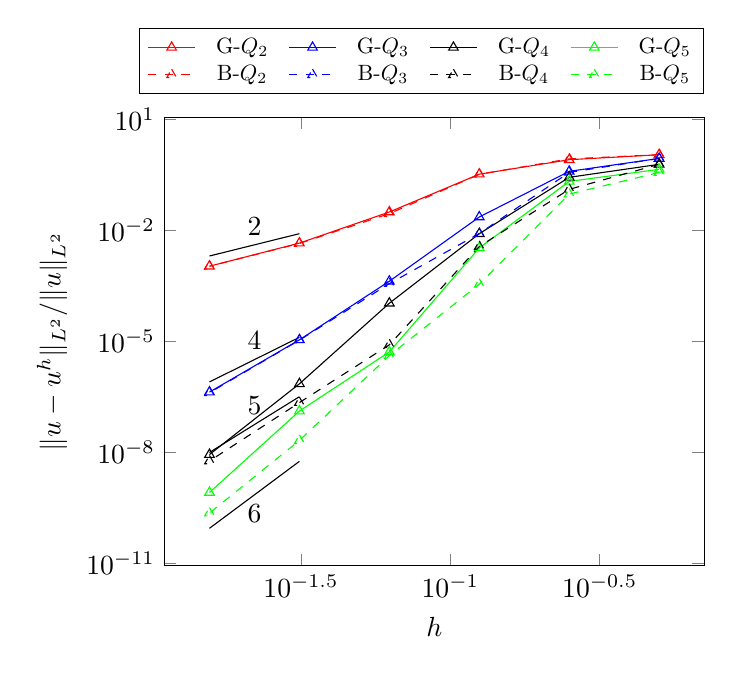
\begin{tikzpicture}
    \begin{loglogaxis}[
        legend columns=4,
    	legend style={at={(1,1.2)}, nodes={scale=0.8, transform shape}, column sep=.2cm},
        xlabel=$h$,
        ylabel=${\|u-u^{h}\|_{L^2}}/{\|u\|_{L^2}}$ 
    ]


    \addplot [color=red,mark=triangle] plot coordinates {

        (.5,    1.08115)
        (.25,   0.792129)
        (.125,   0.322907)
        (.0625,   0.0307356)
        (0.03125,   0.00444968)
        (0.015625,   0.00106043)
    };

    \addplot [color=blue,mark=triangle] plot coordinates {

        (.5,    0.857518)
        (.25,   0.385025)
        (.125,   0.0225406)
        (.0625,   0.00041709)
        (0.03125,   1.09308e-05)
        (0.015625,   4.26084e-07) 
    };

    \addplot [color=black,mark=triangle] plot coordinates {

        (.5,    0.595125)
        (.25,   0.265113)
        (.125,   0.00797683)
        (.0625,   0.000106357)
        (0.03125,   7.13069e-07)
        (0.015625,  8.78607e-09 )
    };

    \addplot [color=green,mark=triangle] plot coordinates {

        (.5,    0.435502 )
        (.25,   0.20598 )
        (.125,   0.00330122)
        (.0625,   5.16129e-06)
        (0.03125,   1.30976e-07)
        (0.015625,   8.33014e-10)
    };

    
    \addplot [color=red,mark=triangle, dashed] plot coordinates {

        (.5,    1.08115)
        (.25,   0.834959)
        (.125,   0.318748)
        (.0625,   0.0277705)
        (0.03125,  0.00436393)
        (0.015625,   0.0010596 )
    };

    \addplot [color=blue,mark=triangle, dashed] plot coordinates {

        (.5,    0.857518)
        (.25,   0.359827)
        (.125,   0.00807084 )
        (.0625,   0.000358953)
        (0.03125,  1.07221e-05)
        (0.015625,  4.09114e-07)
    };

    \addplot [color=black,mark=triangle, dashed] plot coordinates {

        (.5,    0.595125)
        (.25,   0.125729)
        (.125,   0.0036115)
        (.0625,   8.02087e-06)
        (0.03125,   2.21844e-07)
        (0.015625,  5.87874e-09 )
    };

    \addplot [color=green,mark=triangle, dashed] plot coordinates {

        (.5,    0.359201 )
        (.25,   0.0937847 )
        (.125,   0.000346784)
        (.0625,   4.10663e-06 )
        (0.03125,  2.11333e-08 )
        (0.015625,   2.31939e-10 )
    };

    \addplot [black] plot coordinates {

        (0.03125,       0.008 )
        (0.015625,      .002 )
    } node[pos=0.5,anchor=south]{$2$};

    \addplot [black] plot coordinates {

        (0.03125,       1.2800e-05)
        (0.015625,      8e-7 )
    } node[pos=0.5,anchor=south]{$4$};

    \addplot [black] plot coordinates {

        (0.03125,       3.2000e-07)
        (0.015625,      1e-8 )
    } node[pos=0.5,anchor=south]{$5$};

    \addplot [black] plot coordinates {

        (0.03125,       5.7600e-09)
        (0.015625,      9e-11 )
    } node[pos=0.5,anchor=north]{$6$};

    \legend{G-$Q_2$\\G-$Q_3$\\G-$Q_4$\\G-$Q_5$\\B-$Q_2$\\B-$Q_3$\\B-$Q_4$\\B-$Q_5$\\}
    \end{loglogaxis}
\end{tikzpicture}

\end{document}


% 1.08115   0.970233
% 0.792129   0.630331
% 0.322907   0.347793
% 0.0307356   0.140633
% 0.00444968   0.063464
% 0.00106043   0.0313622

% 0.857518   0.812838
% 0.385025   0.451057
% 0.0225406   0.0804161
% 0.00041709   0.00981443
% 1.09308e-05   0.00214694
% 4.26084e-07   0.000516027

% 0.595125   0.727478
% 0.265113   0.347299
% 0.00797683   0.0382459
% 0.000106357   0.00174571
% 7.13069e-07   9.75601e-05
% 6.78607e-09   1.10561e-05

% 0.435502   0.5517
% 0.20598   0.310648
% 0.00330122   0.0166288
% 5.16129e-06   0.000217162
% 1.30976e-07   1.05336e-05
% 8.33014e-10   3.38835e-07